\chapter{Buying the Playbook}

The interview begins with visible wealth, but the useful lesson is not the house or the cars. It is the movement from labor to ownership, from building everything from zero to buying a working business, and from a vague ambition to a cash-flow test. TJ's claims are interview claims, and the transcript does not give a full underwriting model. Still, it gives us a compact arithmetic of wealth: time is capped, ownership can be uncapped, and leverage only helps when cash flow can carry it.

\section{The Hook and the First Explanation}

The opening uses spectacle to force a question. The interviewer stands in front of a mansion, points to expensive cars, and asks about scale. TJ's answer gives the first pair of numbers:
\begin{equation}
R_{\mathrm{annual}} \approx \$90\text{ million to }\$100\text{ million},
\end{equation}
for annual company revenue across his businesses, and
\begin{equation}
I_{\mathrm{personal}} \approx \$25\text{ million},
\end{equation}
for what he says he made personally.

These are not audited statements; they are claims from the interview. But they establish the object to be explained. We are not trying to infer virtue from possessions. We are trying to understand what kind of economic structure could produce that scale.

TJ's first explanation is ownership. He says his main business was tech services, that he built it and sold it, then built and sold a construction business, and today has a supplement business. He describes himself as owning just under ten companies. The first distinction is therefore simple:
\begin{equation}
\text{salary} \neq \text{ownership of operating businesses}.
\end{equation}
A salary is a payment for work. An owned business is a claim on a system.

\section{No Rich Parents, No Finished Map}

The interviewer next removes the easiest story: inherited wealth. TJ says he did not come from money. His mother was fourteen when she became pregnant with him, and he grew up in the South with food stamps and government cheese. The point is not merely biographical. It sets up the central contrast of the interview: no money at the beginning, but not, in his words, a ``broke mindset.''

He also refuses the clean retrospective myth. He did not know, as a child, that he wanted to build a hundred-million-dollar company. He says he wanted to be successful, wanted to get out of the environment he was in, worked, tried to be useful, and kept redefining success as he grew.

\subsection{Question \& Answer}

\paragraph{Question.} Did TJ begin with a precise hundred-million-dollar target?

\paragraph{Answer.} No. The transcript's rhythm matters here. First comes discomfort with the starting environment; then work, usefulness, and repeated redefinition. The target was not initially a number. It was escape from a condition.

This matters because the lecture-like structure of the interview begins with motivation, not mechanics. We first learn why movement was necessary. Only after that do we learn the machinery.

\section{The First Rule: Time Has a Ceiling}

The first general rule appears when TJ warns against trading dollars for hours. We can write the stripped-down model as
\begin{equation}
I_{\mathrm{labor}} = w h,
\end{equation}
where \(w\) is the hourly rate and \(h\) is the number of hours worked.

The limitation is immediate. A person can raise \(w\), but \(h\) is bounded:
\begin{equation}
h \leq h_{\max}
\qquad\Longrightarrow\qquad
I_{\mathrm{labor}} \leq w h_{\max}.
\end{equation}
This is a simple model, but it captures TJ's claim. If the mechanism is direct labor, income remains tied to the body and calendar of the worker.

That is why the conversation moves from work to systems. TJ says to make money while sleeping, build systems, invest, and create passive income. In our notation, the goal is not merely to increase \(w\). It is to leave the one-person equation:
\begin{equation}
I_{\mathrm{labor}} = w h
\end{equation}
and move toward claims on systems that can operate without every dollar being attached to the owner's immediate hour.

\section{Buying the Playbook}

The interviewer then asks what a person should do now if they are stuck trading time for money and want financial freedom. TJ briefly mentions real estate, but he immediately turns to the answer that drives the rest of the interview: buy businesses.

The phrase he uses is the key: go get the playbook. Most people, he says, want to build a business from scratch. His alternative is to buy something already working. An existing business has customers, process, a history of sales, and some evidence of cash flow. It is not risk-free, but it is not blank paper.

\subsection{Question \& Answer}

\paragraph{Question.} Why buy instead of build?

\paragraph{Answer.} Because, in TJ's framing, buying an operating business means buying evidence. The buyer can see that the business is already working. The playbook is not theoretical; it is in the books, the customers, the routes, the machines, the staff, or the repeat service. The opportunity appears because owners may want to leave, may lack succession plans, or may need cash because of divorce, sickness, fatigue, or age.

\begin{figure}
\centering
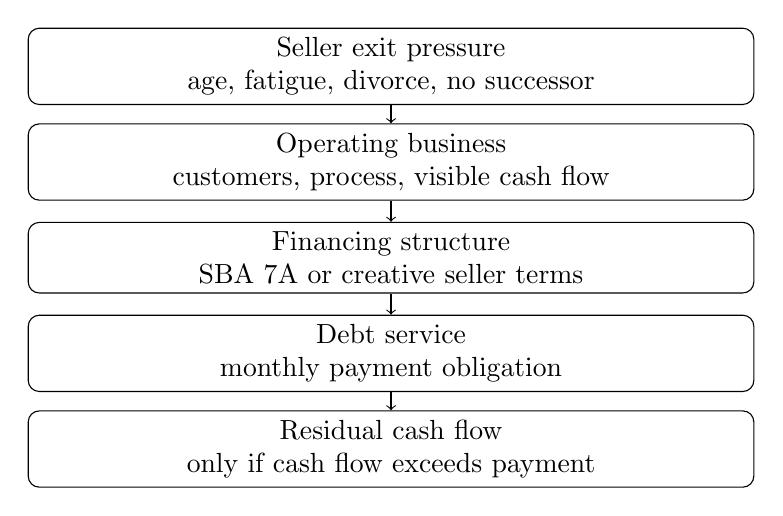
\begin{tikzpicture}[scale=0.90]
\node[draw, rounded corners, align=center, minimum width=0.76\linewidth, minimum height=0.78cm] (seller) at (0,0) {Seller exit pressure\\age, fatigue, divorce, no successor};
\node[draw, rounded corners, align=center, minimum width=0.76\linewidth, minimum height=0.78cm] (business) at (0,-1.35) {Operating business\\customers, process, visible cash flow};
\node[draw, rounded corners, align=center, minimum width=0.76\linewidth, minimum height=0.78cm] (finance) at (0,-2.70) {Financing structure\\SBA 7A or creative seller terms};
\node[draw, rounded corners, align=center, minimum width=0.76\linewidth, minimum height=0.78cm] (service) at (0,-4.05) {Debt service\\monthly payment obligation};
\node[draw, rounded corners, align=center, minimum width=0.76\linewidth, minimum height=0.78cm] (surplus) at (0,-5.40) {Residual cash flow\\only if cash flow exceeds payment};
\draw[->] (seller) -- (business);
\draw[->] (business) -- (finance);
\draw[->] (finance) -- (service);
\draw[->] (service) -- (surplus);
\end{tikzpicture}
\caption{A transcript-grounded reconstruction of TJ's acquisition logic. There is no validated board screenshot for this lecture; the diagram summarizes the spoken mechanism.}
\end{figure}

\section{The Acquisition Arithmetic}

The interview becomes most explicit when the interviewer asks whether this is like private equity. TJ says it is not so much private equity as leveraged buyouts. He does not build a formal finance model, but he gives enough arithmetic to preserve the core test.

Let
\begin{equation}
C_{\mathrm{monthly}}=\text{monthly business cash flow},
\end{equation}
and let
\begin{equation}
D_{\mathrm{monthly}}=\text{monthly debt service}.
\end{equation}
Then the acquisition only begins to make sense if the residual is positive:
\begin{equation}
S_{\mathrm{monthly}}=C_{\mathrm{monthly}}-D_{\mathrm{monthly}}.
\end{equation}

TJ's example is a business that cash flows at \(\$20{,}000\) per month. He then imagines debt service of either \(\$7{,}000\) or \(\$10{,}000\) per month:
\begin{equation}
C_{\mathrm{monthly}}=\$20{,}000,
\qquad
D_{\mathrm{monthly}}\in\{\$7{,}000,\ \$10{,}000\}.
\end{equation}
The resulting surplus range is
\begin{align}
S_{\mathrm{monthly}}
  &= \$20{,}000-D_{\mathrm{monthly}},\\
  &\in \{\$13{,}000,\ \$10{,}000\}.
\end{align}
The clean case in his spoken example is
\begin{equation}
\$20{,}000-\$10{,}000=\$10{,}000.
\end{equation}

\subsection{Worked Example}

Take the higher debt-service case, because it is the one TJ explicitly turns into ``you're up ten thousand.'' The reasoning is:
\begin{enumerate}
\item The acquired business produces \(C_{\mathrm{monthly}}=\$20{,}000\).
\item The acquisition financing requires \(D_{\mathrm{monthly}}=\$10{,}000\).
\item The buyer's monthly surplus is defined by
\[
S_{\mathrm{monthly}}=C_{\mathrm{monthly}}-D_{\mathrm{monthly}}.
\]
\item Substitution gives
\[
S_{\mathrm{monthly}}=\$20{,}000-\$10{,}000=\$10{,}000.
\]
\end{enumerate}

This is the point where the notation must stay humble. The transcript does not define ``cash flow'' as EBITDA, free cash flow, seller discretionary earnings, or net operating income. It uses the term in the loose interview sense: money left by the business that can help carry the purchase. The equation is therefore not a valuation model. It is a discipline: before the buyer celebrates leverage, the buyer must ask whether the business can carry the financing.

\subsection{Question \& Answer}

\paragraph{Question.} When does leverage help rather than trap the buyer?

\paragraph{Answer.} In the interview's arithmetic, leverage helps only if
\begin{equation}
C_{\mathrm{monthly}}>D_{\mathrm{monthly}}.
\end{equation}
If the inequality reverses, the buyer has not bought freedom. The buyer has bought a shortfall. TJ's example shows the attractive case, but the necessary condition is the inequality, not the optimism.

\section{Supply: What to Buy and Where to Find It}

Once the arithmetic is on the table, the interviewer asks the practical questions in the right order. What kind of business? Where do you find one? Why would anyone sell?

TJ names laundromats, pool companies, and vending machine businesses. He likes them because they can cash flow, can be understandable, and may be less dependent on specialized knowledge than a technical startup. He also calls them recession-proof. That phrase should remain an interview claim, not a proven theorem.

\begin{table}
\centering
\begin{tabular}{p{0.24\linewidth}p{0.34\linewidth}p{0.32\linewidth}}
Business type & Why it appears in the transcript & Caution for the notes \\
Laundromat & Cash-flowing local service with a visible operating pattern & Location, machines, repairs, and lease terms still matter \\
Pool company & Recurring service business with route-like demand & Labor, scheduling, retention, and seasonality can matter \\
Vending machines & Simple operating idea with repeat small transactions & Placement, restocking, shrinkage, and machine uptime decide results \\
\end{tabular}
\caption{Transcript-backed examples of acquisition targets. The table preserves TJ's categories while separating claim from operating caution.}
\end{table}

For sourcing, he names three channels: online business-sale portals, business brokers, and cold calls. The cold-call point matters because it changes the picture from passive browsing to active market-making. Some owners may not be listed anywhere, but might sell if a buyer appears.

The broader supply thesis is what TJ calls the ``gray tsunami.'' Older owners may need to exit, and their children may not want to take over. The buyer's opportunity is therefore tied to the seller's problem:
\begin{equation}
\text{succession gap}+\text{seller exit need}
\longrightarrow
\text{acquisition opportunity}.
\end{equation}
This is not merely finance. It is a relationship between a buyer's desire for ownership and a seller's need for transition.

\section{Mindset, Faith, Skill, and Marketing}

After the acquisition section, the interview circles back to the person who has to act on the mechanism. TJ says he has been broke before, and he also says he has gone bankrupt. But he distinguishes being broke in money from having what he calls a broke mindset. In the transcript's rhythm, this is not a slogan inserted at random. It is a recap: the person who would buy, finance, call, negotiate, and operate has to believe action is available.

The same logic appears in the discussion of faith. TJ tells a personal story about belief, then generalizes it: when someone truly believes something, it drives action, thought, and relationships. We can preserve the structure without pretending it is a proof:
\begin{equation}
\text{belief}
\longrightarrow
\text{action}
\longrightarrow
\text{relationships}
\longrightarrow
\text{opportunity}.
\end{equation}

College is treated with similar restraint. TJ says college did not make him a millionaire, but it did not hurt him. It helped him get a skill set: computer programming, and then a job as a computer programmer. Skill matters, but in this interview it is not the whole wealth mechanism. It is one component that can get a person into the game.

\subsection{Question \& Answer}

\paragraph{Question.} What business lesson does TJ say people do not learn in business school?

\paragraph{Answer.} Marketing. His formulation is direct: people may need what you offer, but they do not know who you are. So the entrepreneur's job is to identify those people, get visible, and tell them. In compact form:
\begin{equation}
\text{value}+\text{no attention}\not\Rightarrow\text{growth}.
\end{equation}
The product may be useful, but usefulness alone is not distribution.

\section{Environment and the Expansion of the Possible}

The final movement of the interview is not another spreadsheet. It is a tour. The interviewer and TJ look across Beverly Park, naming nearby houses and large car collections. Treated carelessly, this becomes celebrity trivia. In the logic of the chapter, it is a lesson about environment.

TJ says that once a person sees what is possible, he cannot unsee it. The claim is not that Los Angeles mechanically creates entrepreneurs. It is that exposure can change the constraint set a person carries around in his head:
\begin{equation}
\text{expanded environment}
\longrightarrow
\text{expanded vision}
\longrightarrow
\text{expanded action set}.
\end{equation}

This completes the arc that began with the mansion. At the start, the house was spectacle. At the end, the environment becomes part of the mechanism: a place where the visible examples are larger, the reference group is different, and the imagination is less obedient to the old ceiling.

TJ closes the substantive interview by contrasting wealthy people with a preset ladder. In his view, wealthy people are not simply asking how much a job can pay or how to climb a predetermined structure. They solve problems and create solutions. The chapter's compact summary of the mechanism is therefore:
\begin{equation}
\text{wealth path}
\approx
\text{ownership}
+\text{cash flow}
+\text{attention}
+\text{expanded constraints}.
\end{equation}
This is a note-taking compression of the interview, not a universal formula. Its value is that it keeps the pieces in the order the conversation revealed them.

\section{Summary}

The interview begins with wealth as a scene, then asks what produced it. TJ's answer moves through a sequence: no inherited money, early motivation to escape, refusal to stay inside capped labor income, and a preference for buying operating businesses rather than building every playbook from zero.

The mathematical center is small but important. Labor income is capped by hours:
\[
I_{\mathrm{labor}}=wh,\qquad h\leq h_{\max}.
\]
An acquisition is attractive only if the business can carry the financing:
\[
S_{\mathrm{monthly}}=C_{\mathrm{monthly}}-D_{\mathrm{monthly}}>0.
\]
TJ's example, \(\$20{,}000-\$10{,}000=\$10{,}000\), is not a complete underwriting model. It is a discipline for thinking about leverage.

The remaining pieces are operating conditions: sellers must exist, buyers must find them, belief must turn into action, skill must become useful, marketing must create attention, and environment can expand what a person thinks is possible. That is the interview's useful structure: ownership first, arithmetic second, and mindset only when it is tied back to action.